% !TEX root = ../main.tex

% 中英标题:\chapter{中文标题}[英文标题]
\chapter{排版图片}[Typesetting pictures]

\section{引言}[Introduction]
图应有自明性。插图应与文字紧密配合,文图相符,内容正确。选图要力求精练,插图、照
片应完整清晰。

\section{博士毕业论文双语题注}[Doctoral picture example]

博士毕业论文双语题注如\figref{golfer1}所示。

\begin{figure}[htpb]
\centering
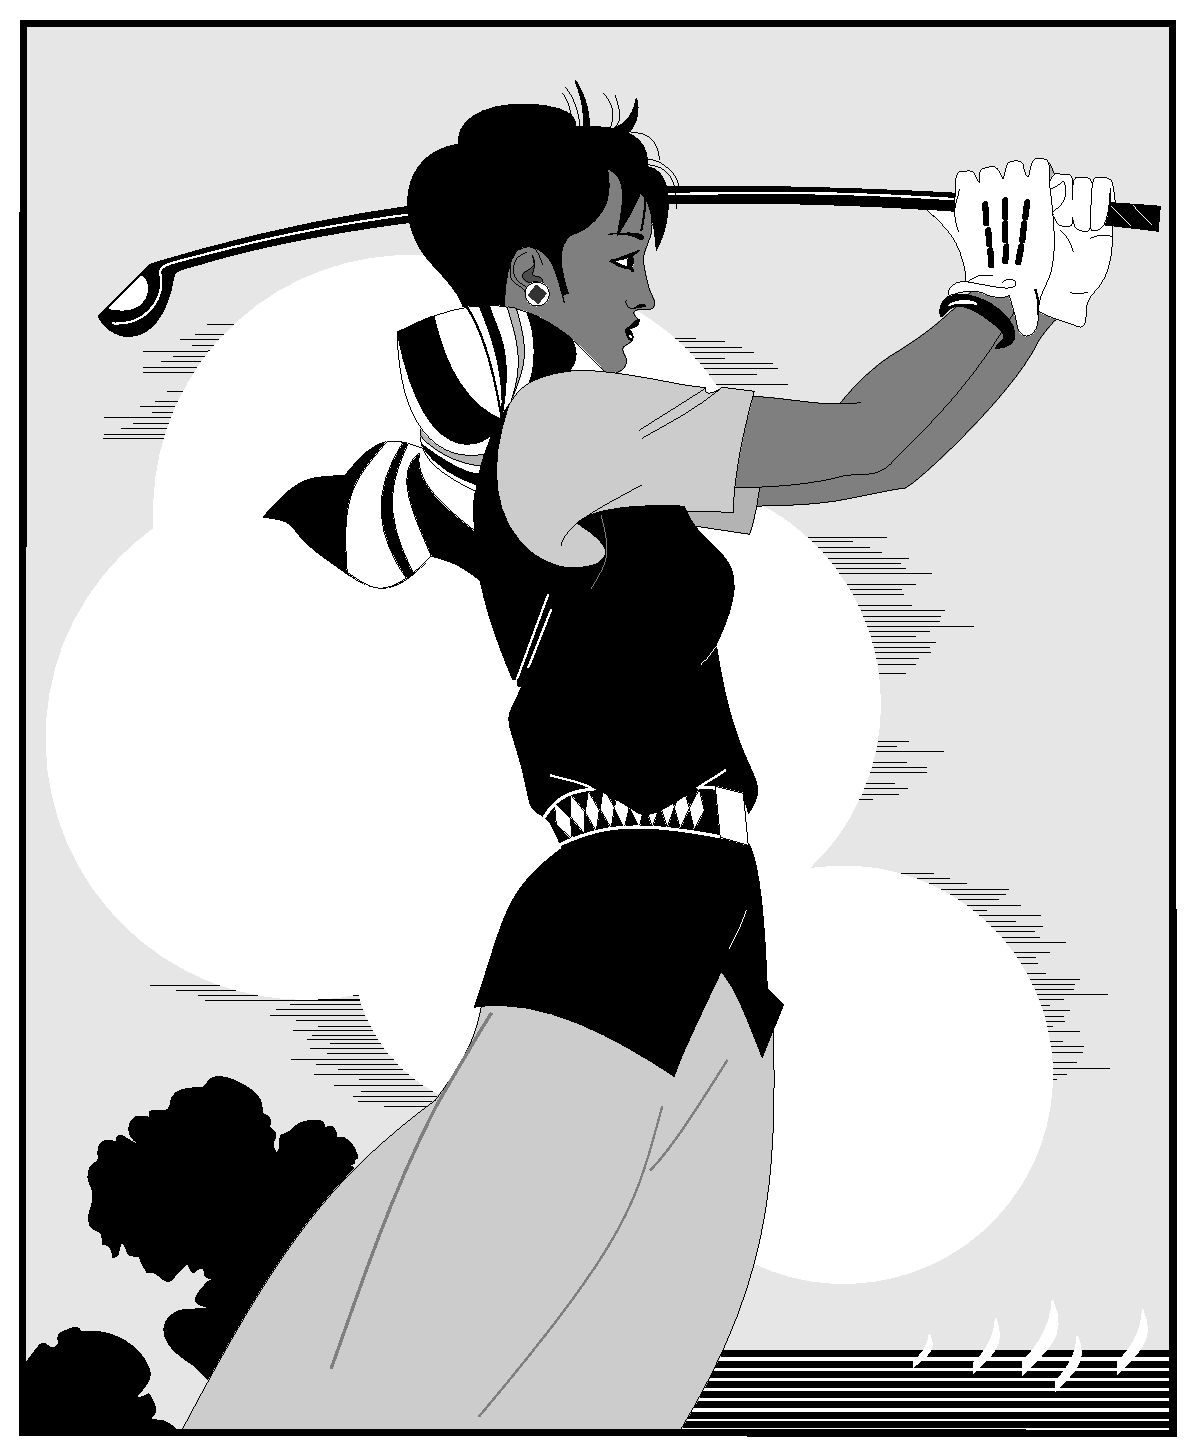
\includegraphics[width = 0.4\textwidth]{golfer}
\bicaption[golfer1]{}{打高尔夫球球的人(博士论文双语题注)}{Fig.$\!$}{The person playing golf (Doctoral thesis)}
\end{figure}

\subsection{内容XXX}[Contents XXX]

\lipsum[3]

\section{内容XXX}[Contents XXX]

\lipsum[2]

\section{本章小结}[Brief summary]

\lipsum[1]
